\documentclass[titlepage, a4paper, 11pt, reqno, openany]{article}%report
\usepackage{amsfonts}
%\usepackage[brazil]{babel} %linguagem do documento
%\usepackage{babel}
\usepackage[portuguese]{babel}
\usepackage{babelbib}
%\usepackage[utf8]{inputenc} %reconhece acento e cedilha
\usepackage{amssymb}
\usepackage{latexsym}
\usepackage{amsmath}
%\usepackage[fleqn]{amsmath}
%\usepackage{mathtools}
%\usepackage[fleqn]{mathtools}
\usepackage{pxfonts} %permite simbolos matemáticos
\usepackage{mathrsfs} %permite uso de fontes para conjuntos
\usepackage[normalem]{ulem} %permite sublinhar palavras
\usepackage{mathrsfs} %permite o uso de letras trabalhadas
%\usepackage[margin=1in, paperwidth=8.5in, paperheight=11in]{geometry}
%\usepackage[top=1in, bottom=1in, left=1in, right=1in]{geometry}
%\usepackage{fullpage}
\usepackage[top=1.5cm,left=1.5cm,right=1.5cm,bottom=1.5cm]{geometry} %margens
\usepackage{graphicx} %permite inserir figuras
\usepackage[usenames]{color} %permite letras coloridas
\usepackage{makeidx} %pra criar índice remissivo
%\usepackage{tikz}
%\usepackage{pgfplots}
\usepackage{mathptmx}
%\usepackage{named}
\usepackage{enumerate}
%\usepackage{amscls}
%alguns pacotes nao sao reconhecidos, ter atencao quais usar em differents computadores.
\usepackage{float}
\usepackage{caption}
\usepackage{verbatim}
%%%%%%%%%%%%%%%%%%%%
\newtheorem{theorem}{Theorem}
\newtheorem{lemma}{Lemma}
\newtheorem{definition}{Defini\c{c}\~{a}o}
\newtheorem{notation}{Notation}
%%%%%%%%%%%%%%%%%%%%

\bibliographystyle{babplain}

\makeindex

%%%%%%%%%%%%%%%%%%%%%%%%%%%%%%%%%%%%%%
\begin{document}
\begin{titlepage}
\begin{minipage}{0.95\linewidth}
\centering

\includegraphics[scale=0.60]{./image/ISEP_marca_cor_grande.png}
\label{Capa}
\title{Electr\'{o}nica de Pot\^{e}ncia}
\author{\emph{S\'{e}rgio Santos},\;$N^o$:\; 1020881}
\date{\today}
\maketitle
\end{minipage}
\end{titlepage}
%titlepage
\pagestyle{plain}%plain headings empty
\tableofcontents
\newpage
%%%%%%%%%%INICIO%%%%%%%%%%%%%%%%%%%%
{\huge Montagens $P2$ e $PD2$.}\par
%
\begin{flushleft}
Considere a seguinte montagem $P2$ da Figura \ref{grafico 1} Suponha $V_s$ = tens\~{a}o da rede el\'{e}ctrica nacional ($230V\,\, 50Hz$).\par
\end{flushleft}
%
%{\Huge $\phi_n \approx$}\\

%{\Huge $\alpha =$}
%
\begin{figure}[H]
\centering
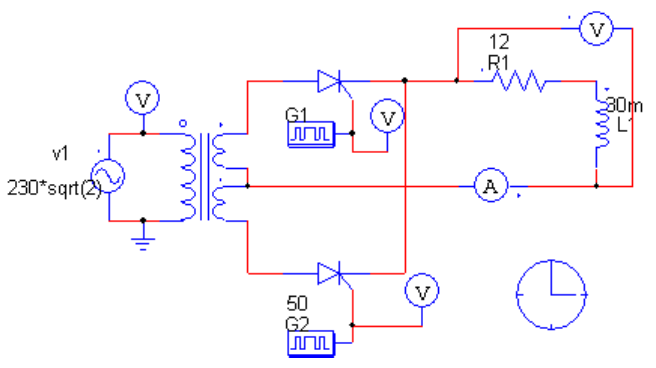
\includegraphics[width=0.75\linewidth]{./image/P3A1.png}\\
\caption{Montagem paralela dupla controlada}
\label{grafico 1}
\end{figure}\par
%seccao 1
\section{\textnormal{Suponha o transformador ideal, com a rela\c{c}\~{a}o de transforma\c{c}\~{a}o entre enrolamentos de $1:1$ e 
que o \^{a}ngulo de disparo dos tir\'{i}stores \'{e} aos $100^{\circ}$ graus.}}\par
%
$R=12\Omega; \qquad L=30\times 10^{-3}\mathbb{H}$\par
Dados passivos do circuito, como constitui de os elementos $RL$ em serie, podemos adquirir a constante de tempo $\tau=\frac{L}{R}$ a sua imped\^{a}ncia $\overrightarrow{Z}=R + j \omega L$ e o desfazamento de regime permanente $\phi_p=\arctan(\frac{\omega L}{R})$.\par
%
Nos \'{e} dado o \^{a}ngulo de disparo de $\alpha=100^{\circ}$ graus e que o circuito tem alimenta\c{c}\~{a}o da rede el\'{e}trica, daqui sabemos que a frequ\^{e}ncia \'{e} de $50 Hz$ e $V_{m\acute{a}x}=230$ da sinusoide. Respetivamente adquirimos a velocidade \^{a}ngular $\omega=2\pi50$ rad/sec.\par
%
Com o \^{a}ngulo de disparo podemos calcular o avan\c{c}o da corrente em regime transit\'{o}rio para isso $\omega t$ \'{e} calculado para $C_T \; e^{\frac{R}{\omega L}*\omega t} = - \frac{V_{m\acute{a}x}}{\overline{Z}}\sin(\omega t + \alpha - \phi)$ 
 no intervalo $[0 \; , \; 2\pi]$ como demonstra na sec\c{c}\~{a}o \ref{eq}. 
$\omega t=1,99219957 \approx 1,990$ radianos, e a corrente \'{e} positiva no intervalo respetivo $0^{\circ} \leq \omega t \leq 114,019^{\circ}$ em refer\^{e}ncia ao disparo.\par
$\phi_n \approx 0,596$ radianos de avan\c{c}o no regime transit\'{o}rio. E $\phi_p \approx 0,666$ radianos no regime permanente mas neste caso s\'{o} nos interessa o transit\'{o}rio.\par
Mais coisas a considerar \'{e} que os tir\'{i}stores s\~{a}o alimentados por fontes em opposi\c{c}\~{a}o de fase, isto quer dizer que os disparos devem estar desfazados de $\pi$ radianos e ter disparo com \^{a}ngulo superior a $\phi_n$.
O sincronismo dos disparos \'{e} crucial para um bom controlo, pois se o segundo tir\'{i}stor disparar enquanto o primeiro esta em condu\c{c}\~{a}o dentro do intervalo $[0 \; , \; \pi]$ o segundo tir\'{i}stor n\~{a}o entra em condu\c{c}\~{a}o, mas se o disparo \'{e} efetuado no intervalo de $[\pi \; , \; \pi+\phi_n]$ este entrara em sobrecarga, pois as condi\c{c}\~{o}es iniciais n\~{a}o ser\~{a}o nulas.\par
%1.1
\subsection{\textnormal{Determine o \^{a}ngulo e o tempo de condu\c{c}\~{a}o $\gamma$ de cada tir\'{i}stor (especifique a express\~{a}o da corrente e determine o tempo de condu\c{c}\~{a}o com a ajuda do {\bf Excel1});}}
%
Representa\c{c}\~{a}o gr\'{a}fica do primeiro disparo, o segundo disparo sera exatamente igual, em que a onda sinusoidal em vez de come\c{c}ar nos $0$ radianos ira come\c{c}ar nos $\pi$ radianos.
\begin{figure}[H]
\centering
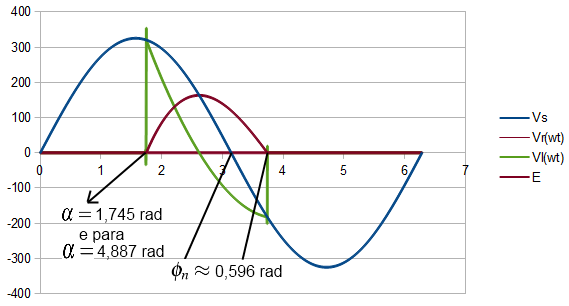
\includegraphics[width=0.75\linewidth]{./image/P3A1_1_3.png}\\
\caption{Representa\c{c}\~{a}o das tens\~{o}es}
\label{grafico 1}
\end{figure}\par
%
O primeiro tir\'{i}stor ira conduzir de $\alpha \approx 1,745$ rad at\'{e} $\pi + \phi_n  \approx 3,738$ rad, e o segundo tir\'{i}stor ira conduzir de $\approx 4,887$ rad at\'{e} $2\pi + \phi_n \approx 6,879$ rad.\par
Cada tir\'{i}store conduz $\gamma \approx 1,993$ rad, que em segundos ser\'{a} $t_c \approx 6,34$ ms num ciclo.
A expressao da corrente \'e como demostrado na se\c{c}\~{a}o \ref{eq}, com $E=0$, isto \'{e},
\begin{equation}
I(\omega t) = \frac{V_{m\acute{a}x}}{\overline{Z}} \sin(\omega t + \alpha - \phi_p) - \frac{V_{m\acute{a}x}}{\overline{Z}} \sin(\alpha - \phi_p) \; e^{-\frac{R}{L \omega}\omega t}
\end{equation}
%1.2
\subsection{\textnormal{Identifique e determine a constante de tempo do circuito.}}
\begin{equation}
\tau = \frac{L}{R} = 2,5 ms 
\end{equation}
%1.3
\subsection{\textnormal{Desenhe numa folha anexa a forma de onda da tens\~{a}o na carga ($V_L$) e uma poss\'{i}vel forma de onda para a corrente ($I_L$) com os respetivos regimes transit\'{o}rio e permanente.}}
%1.4
\subsection{\textnormal{Determine o valor m\'{e}dio da tens\~{a}o $V_{Lo}$, na carga;}}
%
A m\'{e}dia \'{e} sempre calculada para um ciclo, onde o integral de zero \'{e} zero,
%
\begin{flalign}
V_{Loav} =& \frac{1}{T} \; \int_0^T V_L(t) dt &\\
V_L(t) =& L \quad \dfrac{d i_L(t)}{dt} &\\
=& L \quad \left( \frac{R \; V_{m\acute{a}x}}{\overline{Z} L} \; \sin(\alpha - \phi_p) \; e^{- \frac{R}{L}t} + \frac{\omega \; V_{m\acute{a}x}}{\overline{Z}} \; \cos(\omega t + \alpha - \phi_p) \right) & \nonumber \\
=& \frac{R \; V_{m\acute{a}x}}{\overline{Z}} \; \sin(\alpha - \phi_p) \; e^{- \frac{R}{L}t} + \frac{\omega \; L \; V_{m\acute{a}x}}{\overline{Z}} \; \cos(\omega t + \alpha - \phi_p) & \nonumber \\
V_L(\omega t) =& \frac{R \; V_{m\acute{a}x}}{\overline{Z}} \; \sin(\alpha - \phi_p) \; e^{- \frac{R}{\omega L}\omega t} + \frac{\omega \; L \; V_{m\acute{a}x}}{\overline{Z}} \; \cos(\omega t + \alpha - \phi_p) & \\
V_{Loav} =& \frac{1}{\pi+\phi_n - \alpha} \; \left. \int_0^{\pi+\phi_n - \alpha} V_L(wt) dt \right|_{\alpha \approx 1,745}&
\end{flalign}



%1.5
\subsection{\textnormal{Especifique o integral que lhe permite determinar o valor eficaz da corrente $I_{Lrms}$  na carga (n\~{a}o necessita calcular o integral, na aula mas fa\c{c}a-o em casa);}}
%1.6
\subsection{\textnormal{Considerando $I_{Lrms}=6$ A, determine a pot\^{e}ncia dissipada na carga;}}
%1.7
\subsection{\textnormal{Utilizando o {\bf Excel} represente a pot\^{e}ncia atribu\'{i}da \`{a} carga $p(t)$ e determine o factor de pot\^{e}ncia $FP$. Nota: $p(t)=v(t).i(t)$ e $P=V.I.\cos \phi$.}}
%1.8
\subsection{\textnormal{Supondo que existe uma f.c.e.m ($E=100v$) represente as formas de onda da corrente ($I_L$) e tens\~{a}o ($V_L$) na carga.}}
%1.9
\subsection{\textnormal{Suponha que substitui os tir\'{i}stores por d\'{i}odos (montagem PD2) e que a montagem apresenta uma $fcem$ ($E=100v$). Desenhe numa folha anexa a forma de onda da tens\~{a}o na carga ($V_L$) e 
uma poss\'{i}vel forma de onda para a corrente ($I_L$).}}





%seccao 2
\section{\textnormal{{\bf PSIM}}}\label{A2}
%2.1
\subsection{\textnormal{Simule os circuitos referidos da aula anterior ($P2$ e $PD2$) para confirmar todos resultados determinados (apresente todas as ondas incluindo os impulsos \'{a}s gates dos tir\'{i}stores).}}


\begin{enumerate}
\item usar a folha {\bf Excel} que obteve no Problema 3;\par 
\item no relat\'{o}rio dever\'{a} justificar todas os c\'{a}lculos e ondas representadas.
\end{enumerate}
%Resumo
\begin{abstract}
%
resumo
%
\end{abstract}
%Seccao 3
\part{Equa\c{c}\~{o}es} \label{eq}
%
\begin{flushleft}
{\bf Corrente Continua Condi\c{c}\~{o}es \index{Condi\c{c}\~{o}es} iniciais \index{iniciais} nulas \index{nulas}.}\par
\end{flushleft}
 \quad Circuito \index{Circuito} $LC$ em $C.C$:\par
%
\begin{itemize}
\item
$i(t)=\frac{V_{DC}\sqrt{LC}}{L}\quad \sin \left( \frac{t}{\sqrt{LC}}\right)\times u(t)$\par
\item
$V_L(t)=V_{DC}\quad \cos\left(\frac{t}{\sqrt{LC}} \right)\times u(t)$\par
\item
$V_c(t)=V_{DC}\quad \left(1-\cos\left(\frac{t}{\sqrt{LC}} \right) \right)\times u(t)$\par
\item
$\omega_n=\frac{1}{\sqrt{LC}}$\par
\item
$\overline{Z}=\sqrt{(\omega_n L-\frac{1}{\omega_n C})^2}$\par
\item
$\phi_p=\frac{\pi}{2}$\par
porque, $\sin(\omega_n t)= \cos(\omega_n t - \pi/2)$\par
\item
$\tau=\infty$\par
\end{itemize}
%
%%%%%%%%%%%%%%%%%%%%%
\quad Circuito \index{Circuito} $RLC$ em $C.C$:\par
%
\begin{enumerate}
%enum1
\item
Para \quad $C(C R^2-4 L)>0$ \quad (Ra\'{i}zes \index{Ra\'{i}zes} reais \index{reais} diferentes \index{diferentes}) \quad Sobreamortecido \index{Sobreamortecido}.\par
%
\begin{itemize}
\item
$i(t)=\frac{2 V_{DC} C e^{\frac{-tR}{2L}} sinh \left( \frac{t \sqrt{C(CR^2-4L)}}{2CL} \right)}{\sqrt{C(CR^2-RL)}}\times u(t)$\par
\item
$V_R(t)=R\times i(t)$\par
\item
$V_L(t)=L\dfrac{di(t)}{dt}$\par
%
\begin{minipage}{0.95\linewidth}
\makebox[\linewidth]{
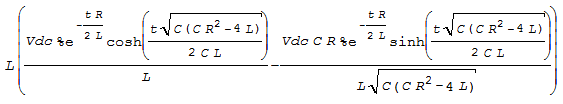
\includegraphics[scale=0.75]{./image/equacoes_1.png}
}
\end{minipage}\par
%
\item
$V_C(t)=\frac{1}{C}\int_0^ti(t)$\par
%
\begin{minipage}{0.95\linewidth}
\makebox[\linewidth]{
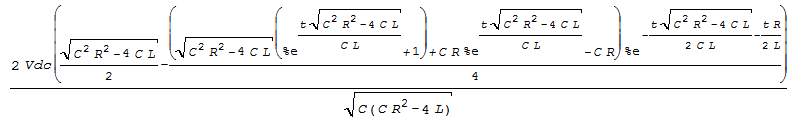
\includegraphics[scale=0.75]{./image/equacoes_2.png}
}
\end{minipage}\par
%
\end{itemize}
%enum2
\item
Para \quad $C(C R^2-4 L)=0$ \quad (Ra\'{i}zes \index{Ra\'{i}zes} iguais \index{iguais})\quad Amortecimento \index{Amortecimento} cr\'{i}tico \index{cr\'{i}tico}.\par
%
\begin{itemize}
\item
$i(t)=\frac{V_{DC}}{L} \quad  t \quad e^{\frac{-R t}{2L}} \times u(t)$\par
\item
$V_R(t)=R\times i(t)$\par
\item
$V_L(t)=L\dfrac{di(t)}{dt}$\par
%
\begin{minipage}{0.95\linewidth}
\makebox[\linewidth]{
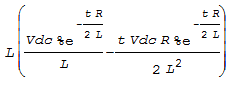
\includegraphics[scale=0.75]{./image/equacoes_3.png}
}
\end{minipage}\par
%
\item
$V_C(t)=\frac{1}{C}\int_0^ti(t)$\par
\begin{minipage}{0.95\linewidth}
\makebox[\linewidth]{
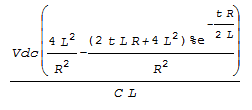
\includegraphics[scale=0.75]{./image/equacoes_4.png}
}
\end{minipage}\par
%
\end{itemize}
%enum3
\item
Para \quad $C(C R^2-4 L)<0$ \quad (Ra\'{i}zes \index{Ra\'{i}zes} complexas \index{complexas}) \quad Amortecido \index{Amortecido}.\par
%
\begin{itemize}
\item
$i(t)=\frac{2 V_{DC} C e^{\frac{-tR}{2L}} sin \left( \frac{t \sqrt{-C(CR^2-4L)}}{2CL} \right)}{\sqrt{-C(CR^2-4L)}}\times u(t)$\par
\item
$V_R(t)=R\times i(t)$\par
\item
$V_L(t)=L\dfrac{di(t)}{dt}$\par
%
\begin{minipage}{0.95\linewidth}
\makebox[\linewidth]{
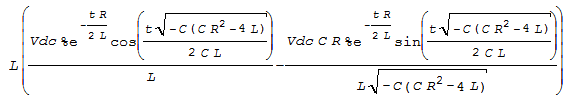
\includegraphics[scale=0.75]{./image/equacoes_5.png}
}
\end{minipage}\par
%
\item
$V_C(t)=\frac{1}{C}\int_0^ti(t)$\par
%
\begin{minipage}{0.95\linewidth}
\makebox[\linewidth]{
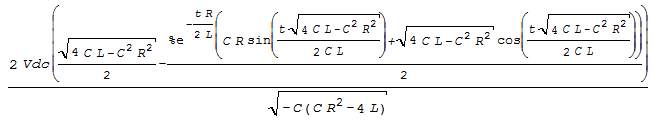
\includegraphics[scale=0.75]{./image/equacoes_6.png}
}
\end{minipage}\par
%
\end{itemize}
\end{enumerate}
%
\begin{itemize}
\item
$| \omega_n |=\sqrt{\frac{4 L-R^2 C}{4 L^2 C}}$\par
\item
%\overrightarrow{Z}
$\overline{Z}=\sqrt{R^2 + (\omega_n L -\frac{1}{\omega_n C})^2}$\par
\item
$\phi_p=\arctan\left(\frac{\omega_n L - \frac{1}{\omega_n C}}{R}\right)$\par
\item
$\tau=\frac{2 L}{R}$\par
\end{itemize}
%%%%%%%%%%%%%%%%%%%%%%%%%%%%%%%%%%%%%%%%%%
\begin{flushleft}
{\bf Corrente \index{Corrente} Alternada condi\c{c}\~{o}es \index{Condi\c{c}\~{o}es} iniciais \index{iniciais} nulas \index{nulas}}.
\end{flushleft}
\quad Circuito \index{Circuito} $RLE$ em $C.A$:\par
\begin{itemize}
\item
$i(t)=C_T\ e^{-\frac{R}{L}t}+\frac{V_{m\acute{a}x}}{\overline{Z}}\sin(\omega t + \alpha - \phi_p)-\frac{E}{R}$\newline
$i(t)=C_T\ e^{-\frac{R}{L}t} + C_1 \cos (\omega t) + C_2 \sin(\omega t)-\frac{E}{R}$
\item
$I(\omega t)=C_T\ e^{-\frac{R}{L \omega}\omega t}+\frac{V_{m\acute{a}x}}{\overline{Z}}\sin(\omega t + \alpha - \phi_p)-\frac{E}{R}$
\item
$\overrightarrow{Z}=R+j\omega L$\\
$\overline{Z}=\sqrt{R^2 + (\omega L)^2}$
\item
$\phi_p=\arctan(\frac{\omega L}{R})$
\item
$C_T=\frac{E}{R}-\frac{V_{m\acute{a}x}}{\overline{Z}}\sin(\alpha - \phi_p)$
\item
$C_T=\frac{V_{m\acute{a}x}}{R^2 + (\omega L)^2}(L \omega \cos(\alpha) - R \sin (\alpha))+\frac{E}{R}$
\item
$C_1=\frac{V_{m\acute{a}x}}{R^2 + (\omega L)^2}(R \sin (\alpha) - L \omega \cos(\alpha))$
\item
$C_2=\frac{V_{m\acute{a}x}}{R^2 + (\omega L)^2}(R \cos (\alpha) + L \omega \sin (\alpha))$
%
\end{itemize}
%%%%%%%%%%%%%%%%%%%%%%%%%%%%%%%%%%
\begin{definition}
Capacit\^{a}ncia
\begin{flalign*}
Q_c(t) =& \int^t i(t) \quad dt & \\
=& Q_c(0^-)+\int_{0^-}^t i(t) \quad dt & \\
V_c(t) =& \frac{Q_c(t)}{C} & \\
=& \frac{1}{C} \quad \int^t i_c(t) \quad dt & \\
=& \frac{Q_c(0^-)}{C} + \frac{1}{c} \quad \int_0^t i_c(t) \quad dt & \\
=& V(0^-) + \frac{1}{c} \quad \int_0^t i_c(t) \quad dt & \\
i_c(t) =& C \quad \dfrac{d V_c(t)}{dt} &
\end{flalign*}\par
\end{definition}
%
\begin{definition}
Indut\^{a}ncia
\begin{flalign*}
\psi_L(t) =& \int^t V_L(t) \quad dt & \\
=& \psi_L(0^-)+\int_{0^-}^t V_L(t) \quad dt & \\
V_L(t) =& L \quad \dfrac{d i_L(t)}{dt} & \\
i_L(t) =& \frac{\psi_L(t)}{L} & \\
=& \frac{1}{L} \quad \int^t V_L(t) \quad dt & \\
=& \frac{\psi_L(0^-)}{L} + \frac{1}{L} \quad \int_0^t V_L(t) \quad dt & \\
=& i_L(0^-) + \frac{1}{L} \quad \int_0^t V_L(t) \quad dt &
\end{flalign*}\par
\end{definition}
%
\begin{definition}
Resist\^{e}ncia
\begin{flalign*}
V_R(t) =& R \quad i_R(t) & \\
i_R(t) =& \frac{V_R(t)}{R} &
\end{flalign*}\par
\end{definition}
%
\begin{definition}
Valor M\'{e}dio
\begin{flalign*}
X_{av} =& \frac{1}{T} \; \int_0^T X(t) dt &
\end{flalign*}\par
\end{definition}
%
\begin{definition}
Valor Eficaz
\begin{flalign*}
X_{ef} =& \sqrt{ \frac{1}{T} \; \int_0^T \overset{\text{2}}{X(t)} dt } &
\end{flalign*}\par
\end{definition}
%

\newpage
\listoffigures
\newpage
\cite{*}
\bibliography{./bibliography/Bibliography}
\newpage
\footnote{Apontamentos Electr\'{o}nica de Pot\^{e}ncia}
%
\end{document}
